\documentclass[10pt]{beamer}
\usepackage[T1]{fontenc}
\usepackage{mathtools}
\usepackage[french]{babel}
\usepackage{amsmath,amssymb,amsthm}
\usepackage{framed}
\usepackage{lmodern}
\usepackage{utils_slides}
\usepackage{pdfpages}
\usepackage{irif}
\usepackage{listings}
\usepackage{listingsutf8}
\usepackage{tikz}
\usetheme{Madrid}
\definecolor{codegreen}{rgb}{0,0.6,0}
\definecolor{codegray}{rgb}{0.5,0.5,0.5}
\definecolor{codepurple}{rgb}{0.58,0,0.82}
\definecolor{backcolour}{rgb}{0.96,0.96,0.95}
\newcommand*{\pmZpmZ }{p^m\Z \x p^m\Z}
\newcommand*{\ZZpmZ}{\Z^2/\pmZpmZ}
\newcommand*{\ZZnZ}{\Z^2/\nZnZ}
\newcommand{\ZpmZ}{\Z/p^m\Z}
\newcommand{\ZZpm}{\ZpmZ \x \ZpmZ}
\newcommand{\nZnZ}{n\Z \x n\Z}
\newcommand{\Mz}{\Set*{
	\begin{pmatrix}
		p^a  & 0   \\
		j & p^b
	\end{pmatrix}
}{
	\begin{aligned}
		 & (a, b) \in A_0      \\
		 & 0 \le j < p^{b}
	\end{aligned}
}}
\newcommand{\Mk}{\Set*{
	\begin{pmatrix}
		p^a  & 0   \\
		jp^k & p^b
	\end{pmatrix}
}{
	\begin{aligned}
		 & (a, b) \in A_k      \\
		 & 0 \le j < p^{b - k}
	\end{aligned}
}}
\newcommand{\Az}{\Set*{(a,b)}{ a + b \le m}}
\newcommand{\Ak}{\Set*{
	(a,b)}{
	\begin{aligned}
		 & a \le m, b \le m \\
		 & a + b = m + k
	\end{aligned}
}}

\title{Sous-groupes de $\ZZ$}
\subtitle{Projet Mathématiques - Informatique}
\author[Kevin Garnier, Charly Martin Avila, Olivier Brunat]{
	\itshape {Kevin Garnier \\
		Charly Martin Avila}\\
		\vspace*{1cm}
	Dirigé par
	Olivier Brunat
}

\date{Année \the\year}
% Top left and top right  Position of a logo in beamer
\titlegraphic {
\begin{tikzpicture}[overlay,remember picture]
\node[left=0.2cm] at (current page.33){
    
\includegraphics[width=3cm]{logo_upc_big.pdf}
};
\end{tikzpicture}
}

\begin{document}
\begin{frame}
	\titlepage
\end{frame}

\begin{frame}
	\frametitle{Matrices à coefficients entier et forme normale de Hermite}
	\begin{block}{Proposition}
		\label{ima_imaq}
		Soient $A \in \M_{m,n}(\Z)$ et $Q \in \GL_n(\Z)$, alors
		$\im AQ = \im A$
	\end{block}
	\begin{alertblock}{Definition}
		Soit $A \in \M_{m,n}(\Z)$. Alors, il existe une unique matrice échelonnée
		réduite suivant les colonnes $H \in \M_{m,n}(\Z)$ telle qu'il existe $Q \in \GL_n(\Z)$
		avec $H = AQ$. La matrice $H$ s'appelle la forme normale de Hermite de A.
	\end{alertblock}
	\begin{example}
		\begin{equation*}
			\begin{split}
				\begin{pmatrix}
					2  & 1  \\
					4  & 10 \\
					5  & 13 \\
					13 & 12
				\end{pmatrix}
				\overset{C_2 \leftrightarrow C_1}{\longrightarrow}
				\begin{pmatrix}
					1  & 2  \\
					10 & 4  \\
					13 & 5  \\
					12 & 13
				\end{pmatrix}
				\overset{C_2 \leftarrow C_2 - 2C_1}{\longrightarrow}
				\begin{pmatrix}
					1  & 0   \\
					10 & -16 \\
					13 & 3   \\
					12 & -14
				\end{pmatrix}
				\overset{C_2 \leftarrow - C_2}{\longrightarrow}
				\begin{pmatrix}
					1  & 0  \\
					10 & 16 \\
					13 & -3 \\
					12 & 14
				\end{pmatrix}
			\end{split}
		\end{equation*}
	\end{example}
\end{frame}

\begin{frame}
	\frametitle{Génération des sous-groupes}
	\begin{alertblock}{Théorème}
		Les seules matrices dont les colonnes génèrent un sous-groupe de $\ZZpmZ$
		sont les matrices de la forme
		$H =
			\begin{pmatrix}
				p^a & 0   \\
				j   & p^b
			\end{pmatrix}
			\text{avec $a \le m$, $b \le m$ et $j < p^b$}
		$
		$ \text{ ou }$
		$ H =\begin{pmatrix}
				p^a  & 0   \\
				jp^k & p^b
			\end{pmatrix}
			\text{avec $a \le m$, $b \le m$, $k \le m$ et $j < p^{b - k}$}
		$
	\end{alertblock}
	\begin{block}{Corollaire}
		Soit la suite $\suit{A}{k}{0 \le k \le n}$ telle que
		$A_0 = \Set*{(a,b)}{ a + b \le m}$\\
		\vspace*{-0.1cm}
		\begin{center}
			$A_k = \Set*{
					(a,b)}{
					\begin{aligned}
						 & a \le m, b \le m \\
						 & a + b = m + k
					\end{aligned}
				}$
		\end{center}

		Alors, l'ensemble des matrices du théorème, \cad, les matrices dont les colonnes
		génèrent les sous-groupes de $\ZZpmZ$ est
		$M = \bigsqcup_{k = 0}^mM_k$
		où \vspace*{-0.1cm}
		\begin{center}
			$
				M_k = \Set*{
					\begin{pmatrix}
						p^a  & 0   \\
						jp^k & p^b
					\end{pmatrix}
				}{
					\begin{aligned}
						 & (a, b) \in A_k      \\
						 & 0 \le j < p^{b - k}
					\end{aligned}
				}
			$
		\end{center}
	\end{block}

\end{frame}

\begin{frame}
	\frametitle{\'Enumération des sous-groupes}
	\begin{alertblock}{Théorème}
		Soit
		\app{\psi}{\N^2}{\N}{(p,n)}{\sum_{i=0}^{n}(n-i)p^i + \sum_{i = 0}^{n}\frac{1- p^{n-i+1}}{1 - p}}
		Alors, le nombre de sous groupe de $\ZZpm$ est $\psi(p,m)$
	\end{alertblock}

	\begin{block}{Proposition}
		Soit $n = \prod\limits_{i = 1}^k p_i^{\alpha_i}$ avec $p_i$ des nombres premiers distincts\\
		Le nombre total de sous-groupes de $\ZZ$ est
		$$\prod_{i = 0}^{k} \psi(p_i,\alpha_i)
			= \prod_i^k\mlarge[3](\sum_{j=0}^{\alpha_i}(\alpha_i-j)p_i^j +%
			\sum_{j = 0}^{\alpha_i}\frac{1- p_i^{\alpha_i-j+1}}{1 - p_i}\mlarge[3])$$
	\end{block}
\end{frame}

\begin{frame}
	\frametitle{Quelques résultats générés}
	\begin{center}
		\begin{tabular}{|c|c|c|c|c|c|c|c|c|c|c|c|}
			\hline
			n       & 0     & 1 & 2 & 3 & 4  & 5 & 6  & 7  & 8  & 9  & 10 \tabularnewline
			\hline
			$|\ZZ|$ & $\oo$ & 1 & 5 & 6 & 15 & 8 & 30 & 10 & 37 & 23 & 40 \tabularnewline
			\hline
		\end{tabular}
	\end{center}


	\begin{figure}[!h]
		\centering
		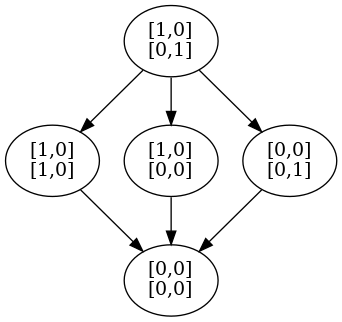
\includegraphics[scale=0.4]{Z2ZxZ2Z.png}
		\caption{
			Treillis des sous-groupes de $\Z/2\Z \x \Z/2\Z$ avec les formes normales de Hermite
			correspondantes
		}
	\end{figure}
\end{frame}
\end{document}
